% An Applied Mathematics/Biology Thesis
% By Jonathan Niles

\documentclass[phd,tocprelim]{cornell}

% packages
\usepackage{natbib}
\usepackage{geometry}
\usepackage{graphicx}
\usepackage{amsmath}
\usepackage{amssymb}
\usepackage{tabu}
\usepackage{longtable}
\usepackage{booktabs}
\usepackage{ifpdf}
\usepackage{appendix}
\usepackage[hidelinks]{hyperref}
\usepackage[toc]{glossaries}

% Set tolerance for box model
\tolerance=9999

% New Commands, refreshers
%\renewcommand{\caption}[1]{\singlespacing\hangcaption{#1}\normalspacing}
\renewcommand{\topfraction}{0.85}
\renewcommand{\textfraction}{0.1}
\renewcommand{\floatpagefraction}{0.75}

% LongTabu Fix
\AtBeginEnvironment{longtabu}{\tiny}{}{}   %% change all longtabu content to foot note size

\title{Structural Indications of Fragility in the Human Genome}
\author{Jonathan Niles}
\conferraldate{June}{2014}
\degreefield{Bachelor of Science}
\copyrightholder{Jonathan Niles}
\copyrightyear{2014}

% Acronym Definitions
\newacronym{dna}{DNA}{Deoxyribonucleic Acid}
\newacronym{rna}{ROA}{Ribonucleic Acid}
\newacronym{geo}{GEO}{Gene Expression Omnibus}
\newacronym{ncbi}{OCBI}{National Center for Biotechnology Information}
\newacronym{sra}{SRA}{Sequence Read Archive}
\newacronym{tad}{TAD}{Topologically Associating Domain}
\newacronym{lad}{LAD}{Lamina Associating Domain}

% Glossary definitions
\newglossaryentry{karyotype}{%
  name={karyotype},
  description={A photomicrograph of chromosomes arranged according to a standard classification.}%
}

\newglossaryentry{polymer}{%
  name={polymer},
  description={A substance that has a molecular structure consisting chiefly or entirely of a large number of similar units bonded together, e.g., many synthetic organic materials used as plastics and resins.}
}

\newglossaryentry{epigenetic}{%
  name={epigenetic},
  description={Any heritable influence on gene activity, unaccompanied by a change in the DNA}
}

\newglossaryentry{restriction enzyme}{%
  name={restriction enzyme},
  description={An enzyme that restricts, or performs double-strand cut, at a specific DNA sequence motif.}
}

\newglossaryentry{ligation}{%
  name={ligation},
  description={The joining of two DNA strands or other molecules by a phosphate ester linkage.}
}

\newglossaryentry{oligonucleotide}{%
  name={oligonucleotide},
  description={A polynucleotide whose molecules contain a relatively small number of nucleotides.}
}

\newglossaryentry{nucleosome}{%
  name={nucleosome},
  description={A chromatin secondary structure consisting of $\sim147$ base pairs of DNA wrapped 1.75 times around an octamer of core histone proteins.}
}

% Make a glossary using the glossaries package
\makeglossaries%

\begin{document}

\maketitle
\makecopyright%

\begin{abstract}
Chromosomal rearrangements and sequence translocations are canonical hallmarks of cancerous cells.  Frequent
occurences of rearrangments at specific loci may give insight into uncharacterised mechanisms that explain
macro-moleclar breaks in the genome.  The canonical models for these `common fragile sites' involve spatially
independent molecular mechanisms of double-strand break repair and non-homologous end joining.  However, the
inherent fragility of genomic compartments may be explained on a structural basis, instead or in addition to,
the biochemical models for sequence rearrangements.  We propose a possible architectural model underlying the
fragility of certain rearranged genes and describe further experiments to understand interplay of form and
disfunction.
\end{abstract}

\begin{dedication}
  This thesis is dedicated to the memory of Miriam P Fountain and Daniel E Fountain.
\end{dedication}

\begin{acknowledgements}
I would like to thank my faculty sponsors for their patience, work ethic, and sympathy:
Dr.\ Tyrone Ryba, Dr.\ Patrick McDonald, and Dr.\ Necmettin Yildirim.
\end{acknowledgements}

\contentspage%
\tablelistpage%
\figurelistpage%

\normalspacing\setcounter{page}{1}\pagenumbering{arabic}
\pagestyle{cornell} \addtolength{\parskip}{0.5\baselineskip}

\chapter{Introduction}

The human genome is a six billion nucleotide string that encodes the
the vast instruction set for the cells growth, function, and death.  The cell
programme is not only dictated by the instruction set, but also
how the instructions are read, compiled, and exectuted, and is influenced
by a myriad of factors in addition to the primary sequence.  Increasingly,
modern cancer research is indicating this epigenetic landscape plays strategic
role in determining cell fate.  Understanding the landmark epigenetic features,
the conditions which bring about their development, and the impact they have on
the cell is of paramount importance and difficultly.

% Mat
\chapter{Mathematical Preliminaries}

This thesis endeavors to secure a relationship between chromatin structure and fragility that may potentially exacerbate or lead to
disease states.  The analysis will include gene expression profiles, iterative curve fitting, and principal component analysis.  This
beginning will serve as an introduction to the numerical methods used to compare and contrast gene expression and chromatin states
between the two cell lines examined within.

\section{Expression Profiling}

The set of genes expressed in a cell, collectively known as the \textit{transcriptome}, provides insight into chromatin accessibility
and cell state.  A gene expressed in $n$ conditions (or $n$ samples) forms vector in $n-$dimensional space.  Similarly, the expression
profile the entire transcriptome for a single sample is a vector in $m-$dimensional space, where $m$ is the number of genes assessed.
We therefore denote an experiment interrogating $n$ genes across $m$ samples as an $m \times n$ matrix $S_{m,n}$.
\[
  S_{m,n} = \left[
    \begin{array}{ccc}
      s_{1,1} & s_{1,2} & \cdots & s_{1,n} \\
      s_{2,1} & s_{2,2} & \cdots & s_{2,n} \\
      \vdots & \vdots & \ddots  & \vdots \\
      s_{m,1} & s_{m,2} & \cdots & s_{m,n}
    \end{array}
  \right]
\]

and a single gene's expression profile is
\[ G_{i} = \begin{pmatrix} g_{i1} & g_{i2} & g_{i3} & \cdots & g_{in} & \end{pmatrix} \]

We wish to compare differences in gene expression profiles for particular, or all, genes between samples.  This amounts to comparing
\textit{distances} between gene expression vectors.  There are several methods for doing so.

The simplest genometic distance measure is \textbf{Euclidean} distance.  Euclidean distance is a particular \textif{norm}, known as
the 2-norm.  Geometrically, the norm is a measure of `size' or `proximity' in $n-$dimensional space.  The 2-norm for a vector $x$ is
defined as
\[
  \|x\|_{2} = {(|x_1|^2 + |x_2|^2 + \cdots + |x_n|^2)}^{\frac{1}{2}}
\]

The distance between two vectors in a vector space can now be found using the triangle inequality on the 2-norm.  As a norm, the Euclidean
norm has some desirable properties, notably, non-negativity, positivity, and a definition of the triangle inequality $\|x + y\| = \|x\| + \|y\|$.
Directly from the triangle inequality, we define the Euclidean distance in $n-$dimensions to be

\[
  D_{Euc}(x,y) = \|x\| - \|y\| = {(\sum_{i=1}^{n}{(a_i - b_i)}^2)}^{\frac{1}{2}}
\]

A second 

% biology chapter
\chapter{Biological Preliminaries}

\section{Building from the Basics}

It is difficult to overstate the importance of chromatin topology in
every aspect of a eukaryotic cell's life.  The morass of nucleic acids and
proteins packed tightly inside the nuclear envelope contains all the
information necessary for cell function and duplication.

The sheer complexity of the nucleus requires us to investigate its biological
structure at multiple layers of granularity.  Ironically, the smallest resolution
of the nucleus is also the most well studied: the primary sequence of nucleic
acid bases which compose the DNA molecule itself.  One level of abstraction
above the primary sequence considers the interactions of the primary sequence
with architectural proteins such as histones, and the secondary structures that
result from these couplings.  Even higher up the abstraction tree lies
\textit{epigenetics} (literally `above genetics'\cite{dictepi2014}), a loose
classification for secondary modifications to DNA and architectural proteins
which may be heritible or characteristic of cell state.  Finally, chromosomes
and chromosomal territories comprise the highest and most recently understood
levels of nuclear architecture.  Conceptualizing nuclear organization in
stata such as this furnishes researchers with a conceptual tool to model
and categorize the topology of nuclear contents.

\subsection{The Primary Sequence}

The fundemental informational unit of the cell is the nucleotide, often
termed base or base pair when joined in a molecule or strand.  Eukaryotic
cells have a principle four character alphabet of nucleotides, distinguished
by their \textit{nucleobases}: adenine, cytosine, guanine, and thymine.  These
nucleotides are affixed to a phosphate backbone into a long, coiling polymer
chain.  The famous publication of the structure of DNA in 1953 by researchers
Watson and Crick demonstracted these polymers exist in the nucleus as double
helices\cite{watson1953}, with hydrogen bonds holding the opposing strands
together.  Adenine and guanine are purine bases, while thymine and cytosine are
pyridine bases.  It is important to note that adenine and thymine are
complementary bases and form two hydrogen bonds between them.  Similarly,
guanine and cytosine are complementary, and form three hydrogen bonds between
their bases.  In this fashion, one particular side of the helix completely
determines the oppsing side and perturbations from this structure may lead
to strand mutations\cite{cox2008}.

One cannot ignore the consituents of the primary sequence, particularly when
considering macroscopic properties of the genome.  The order and
nucleotide content can change the local flexibility and directly (by
encoding binding sites) and indirectly (by supporting the binding of histones)
modulates the binding of important architectural proteins\cite{travers2004}.
Although a DNA strand is a helical structure, it is an intrinsically
flexible molecule.  A naive calculation reveals that the human genome is
roughly two meters in length%
\footnote{%
  A diploid human genome consists of two copies of the $\sim3.1MB$ DNA molecule,
  based off estimates from the OCBI human genome reference build 37.
  Each base pair is assumed to ce roughly $0.34\times10^{-9}m$.  Therefore, the
  entire length is $2(0.34 \times 10^{-9})(3.2 \times 10^9) = 2.176m$
},
yet the entire genome fits into a nuclear volume of $\sim523\mu{}m$
\cite{marks2011}.  Furthermore, loops as small as 100 bases in length have been
reported in enhancer and repressor element activation pathways\cite{wong2008}.
These loops can form independently of proteins\cite{vafabakhsh2012}.  Altogether, DNA's
inherent flexibility is the foundation for  many complex higher order
chromatin structures.

%% FIXME DNA METHLYATION
\textbf{TODO: DNA METHYLATION}

\subsection{Epigenetics And Chromatin Modeling}

How a DNA molecule is packaged and condensed within a cell nucleus remains
one of the basic questions of cell biology.  Intellectual curiousity aside,
why is it so important to unravel the chromosomal architecture?  J.C. Hansen
notes, `In biology, structure is inexorably linked to function.'\cite{hansen2012}
The pursuit of an accurate \textit{in vivo} model for DNA and protein packaging
continues to persist today, despite a legacy of experimental, conceptual, and
mathematical models.

In 1974, Kornberg discovered that chromatin contained roughly equal amounts of
DNA and protein\cite{kornberg1974}.  A year later, Pierre Chambon and collegues
described the separation of chromatin into protein complexes spaced evenly on the DNA
molecule as `beads on a string.'\cite{oudet1975}  The observed beads are nucleosomes,
bundles composed of a histone octamer and $\sim200$ bases (later reported to be
$167$ bases\cite{robinson2006}) of coiled DNA\@.
Much as the nucleotide is the fundemental unit of the genome, nucleosomes are
the fundemental units of the epigenome.  Nucleosomes in series are called a
nucleosome array.  A nucleosome consists of two components: a core particle
wrapping $\sim146$ base pairs of DNA, yeilding a 6 fold compaction in length,
and a linker portion of varying length of $0$ to $\sim80$ base pairs.  The
linker component connects adjacent nucleosomes in a nucleosome array\cite{wu2007}%
\cite{hansen2012}.  These arrays are $10-nm$ in diameter, provoking them to be
often called the `$10-nm$' fibers.

Despite decades of research on nucleosome arrays, their structural conformation
\textit{in vivo} remains enigmatic.   Does another higher order structure exist
beyond the $10-nm$ fiber?  Nucleosome arrays and linker histones suspended in ionic
solution fold naturally into a $30-nm$ fiber\cite{tremethick2007}; however, it
is unclear whether this motif forms \textit{in vivo} and its conformation may
be different in the nuclear context\cite{bian2012}.  The $30-nm$ fiber model
is appealing as it readily explains the highly compacted structure of mitotic
chromosomes.  To form the fiber, arrays of nucleosomes are arranged in a
solenoid or double-helix structure (for full review, see Grigoryev and
Woodcock\cite{grigoryev2012}).  Whether one or both structures are present in
sub-chromosomal architectures is still an open question\cite{song2014}.  Recently,
experiments using cryogenic electron microscopy (cryo-EM) suggested an
alternative fractal arrangement of $10-nm$ fibers, without invoking a higher
organizational unit\cite{nishino2012}\cite{hansen2012}.  It likely that a
mixture of these organizational schemas exist \textit{in vivo}.  Further
research as needed to assess the biological relevance of the $30-nm$ fiber in
both interphase and mitotic chromosome structure.

The nucleosome core particle is a central actor controlling gene expression
through local transcription regulation.  It is well established that nucleosomes
cause an attentuation of gene expression when present at physiological
concentrations\cite{brown1984}\cite{lorch1987}\cite{laybourn1991}\cite{juan1994}.
How then does the cell maintain some genes as actively transcribed while others
are silenced?  Nucleosomes regulate gene expression by regulating accessibility.
Gene expression is mediated by a confluence of protein-DNA interactions:
enhancers bind to enhancer elements, polymerases to the transcription start
site (TSS), and polymerase recruitment proteins line the promoter region to
facilitate polymerase binding and transcription activation\cite{cox2008}.  At
any protein-DNA junction, local chromatin compaction can exclude binding by
physically restricting access to the primary sequence.  This tightly packed
form of DNA is called \textit{heterochromatin}, while open and accessible
sequence is called \textit{euchromatin}.

\textbf{TODO}
A critical feature of gene regulation is the ability to form long range
interactions between distal elements of the genome.  Note, cite heintzman et al.

\subsection{Chromosomes are organised in territories}

The highest level of genome organization is the chromosome territory (CT) or chromosome neighboorhood\cite{cremer2001}.
The hypothesis that chromosomes were segregated into nuclear subvolumes dates back more than 100
years\cite{cremer1993}.  The raison d'etre of these territories is not well understood; however, it is
proposed that CT distribution in the nucleus protects the gene-rich chromosomes by localizing them to
the nuclear center\cite{boyle2001}\cite{federico2006}, CTs create gene expression `pockets' with localized
transcriptional and repair machinery\cite{bolzer2005}, and may have cell type specific positioning.

% TODO Are the chromosomal territories inherited throughout progeny?
% http://ac.els-cdn.com/S0092867403001892/1-s2.0-S0092867403001892-main.pdf?_tid=ccd0bd28-a889-11e4-9e90-00000aab0f26&acdnat=1422627232_949e19f69451fec3a919f3039a1c2a70

To date, there is no evidence to support a deterministic ordering of chromosomes in the nucleus.  However,
there may exist certain deterministic rules to chromosomal positioning.  In all human cell types studied,
the radial position of the chromosomes is correlated with gene density and chromosome size\cite{sun2000}\cite{bolzer2005}.
In most cell types, gene-rich chromosomes are found in the central nuclear compartment, while gene-poor
chromosomes surround the nuclear periphery\cite{boyle2001}\cite{kozubek2005}.  However, in cell types with
non-spherical nuclear shapes, chromosomal arrangements may deviate from this pattern, possibly reflecting
more specialized functions\cite{bolzer2005}.

There is strong evidence that chromosomal territories contain small decondensed regions serving as gene
expression hotspots.  Unlike bacterial chromosomes, where genes from the same pathway are grouped on the
chromosome in units called \textit{operons}, eukaryotic genes are distributed seemingly randomly thoughout
the genome\cite{jacob1961}.  It is well known that transcriptionally active chromatin compartmentalizes based
on replication timing\cite{ferreira1997}\cite{sadoni1999}\cite{thevenin2014}.  Moreover, recent obervations
reveal in order to facilitate transcription of genes in a pathway, chromosomal territories co-localize
functionally related genes with transcriptional machinery.  When considering only inter-chromosomal gene pairs,
Thevenin and collegues observed that co-functioning genes exhibit significant local concentrations, regardless
of linear distance on the primary sequence\cite{thevenin2014}.

% TODO Topologically associated domans?
% http://www.ncbi.nlm.nih.gov/pmc/articles/PMC3874840/

% TODO
% What is this about chromosome neighboorhood location determines translocation outcome?

\chapter{Chromosomal Conformational Capture and Derivatives}

\section{Capturing Conformations}

The field of molecular biology is advancing rapidly, propelled forth by a
surge of automated techniques.  These so-called `high-throughput' methodologies
enable biologists and bioinformaticians to generate massive datasets with
relative ease, reliability, and efficiency.  The first reference build of the
human genome is a testament to their success\cite{hgsc2004}.  However,
until recently, investigating chromosomal architecture remained an
exhaustively manual process, relying on flourescence microscopy experiments and
visual inspection by researchers.  It was not until 2003, when Job Dekker and
collegues described a technique known as Chromosomal Conformational Capture
(3C) that the study of nuclear architecture gained a high throughput methodology
\cite{dekker2002}. Since then, a family of high-throughput capture techniques,
most named a variation on `3C', have been developed to interrogate
different scales and types of chromatin interactions.

The original chromosome conformation capture technique developed by Dekker and
collegues provides an average measurement of the juxtaposition frequency between
two specific genomic loci in a cell population\cite{frase2014}.  This
interaction frequency measurement is thought to be reflective of the distance
between two associated loci in genomic space.  The first extension of the 3C
experiment, aptly named Chromosome Conformation Capture-on-Chip (4C), increased
the number of interrogated regions from two loci (one to one) to all loci
interacting with a chosen target region (one to all)\cite{simonis2006}.  Most
recently, the Dekker lab extended the method further using biotinylated probes
to assess contacts across the entire genome (all to all)\cite{berkum2010}.
The method, known as Hi-C, boasts the first truly global quantization of every
genomic contact at a given time.

The conceptual idea behind chromosomal conformation capture is remarkably
simple --- to assess nearby regions, the experimenter attempts to fuse
together molecules that are physically close, then determine the interaction
partners of each segment of DNA captured in this fashion.  The 3C proceedure
involves five steps.   Initially, a population of cells is cultured in an appropriate
growth medium to a population size of $\sim2.5 \times 10^7$ cells\cite{berkum2010}.
The entire population is treated with formaldehyde, a small chemical commonly
used to fix both cellular samples for microscopy experiments and large specimens
for organismal analysis.  Formaldehyde is a mutagen known to form DNA-DNA and
DNA-protein crosslinks\cite{merk1998}.  Importantly, the formaldehyde
treatment covalently binds together proximal DNA and protein structures.
In the second step, the cells are homogenized and chromatin is digested by a
restriction endonuclease, an enzyme that create double-strand cuts at certain
base pair sequences\cite{berkum2010}.  Digestion creates two populations of
DNA fragments: fragements bound to protein/DNA complexes, and an unbound
population.  The unbound population is discarded by filtering.  In the
third step, the bound double-strand sequences are ligated, or joined together,
in highly diluted concentrations. Dilution is critical to ensure ligation
reactions occur only between DNA strands bound to the same molecular complex.
The result of the ligation process is a population of chimeric DNA sequences.
The fourth step reverses the crosslinks and release the recombined sequences
from their complexes.  The final step comprises quantifying the restriction
fragments by PCR using primers specific for the population under
study\cite{simonis2007}.

\textbf{TODO}
%
% FIXME
%   The 4C protocol is not very well understood.  Please round out this
% knowledge and fill in the section appropriately.
%

In the derivative methods 4C, 5C, and HiC, the basic protocol remains
unchanged; however, the capture and analysis of chimeric fragments varies
depending on the application.  Chromosome Conformation Capture-on-Chip (4C)
leverages a DNA microarray to systematically screen the entire genome in an
unbiased manner for DNA loci that contact a single locus\cite{simonis2006}.
The microarray is tiled with probes which match sequences $< 100$ base pairs
away from a restriction site.  Instead of performing the PCR step from the
canonical 3C assay, restriction fragments are shortened with a second restriction
enzyme, circularized, and amplified by inverse PCR\@.  Amplified probes
are detected by microarray\cite{simonis2006}.  Chromosome Conformation Capture Carbon-Copy (5C)
extends the 3C method by replacing the PCR amplification step with multiplexed
ligation-mediated amplification.  Ligation-mediated amplification (LMA) is a
technique to detect and amplify specific target sequences using primer pairs
that anneal next to each other on the same DNA strand\cite{dostie2006}.
Critically, the 5C method only amplifies strands which are bound by two
primers ligated across the DNA ligation junction, allowing fine control over
the amplified sequences through primer careful design.  Primers are
designed such that forward and reverse 5C primers are ligated across ligation
junctions of select loci in the 3C library.
Furthermore, 5C primers also contain universal tails for amplification,
permitting all bound sequences to be simultaneously amplified.  Thus, through
the appropriate choice of primers, a selected genomic loci is `carbon-copied'
and amplified, allowing high resolution analysis of a given target
interaction\cite{dostie2006}.  The most recent derivation of the technique,
HiC, allows comprehensive capture of all interacting segments in the genome
using Next Generation Sequencing (NGS) techniques.  To purify all interacting
segments of the genome, the HiC protocol calls for the labeling of all junctions
with biotin markers, effectively marking each genomic junction. Like other
derivative methods, HiC abolishes the PCR step of 3C and replaes it with filtration
using steptavidin beads to pull down chimeric DNA sequences.  The captured sequences
can then be sequenced using next generation sequences or hybridized to a
microarray.  More targeted methods ChiA-PET and ChIP-loop encorporate
immunoprecipitation to select complexes containing certain proteins.


\begin{figure}[b]
  \centering
  \caption{An overview of 3C methods.}
  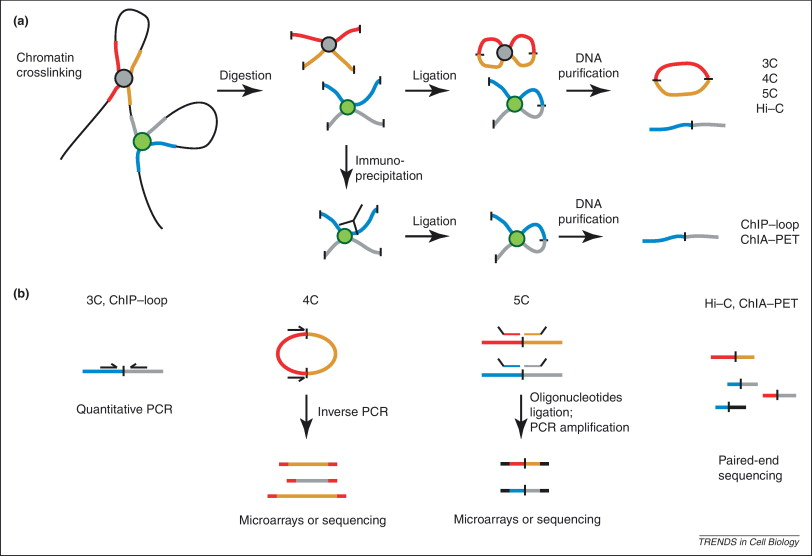
\includegraphics[width=\textwidth]{figures/CompareChromosomeCapture}
  \medskip
  \small
  Chromatin is uniformly crosslinked and digested with a restriction enzyme.
  Bound sequences are immunoprecipitated or biotinylated, depending on the
  assay, and strands are ligated.  Ligation yeilds novel chimeric sequences
  which are purified.  The number of interactions are assess by qPCR in
  the canonical 3C method and ChIP-loop, inverse PCR in 4C, multiplexed
  sequencing with oligonucleotides in 5C, and paired end sequencing in Hi-C
  and ChIA-PET\@.  Adapted from Montavon \textit{et al.}\cite{montavon2012}.
\end{figure}


\section{Analysis}

The perceptive reader will note that much can go wrong in a 3C experiment.
Every 3C method involves some level of digestion, ligation, and amplification,
and errors may be introduced at each step.  In particular, Dekker provides
guidelines for three important control steps to ensure the methodology remains
integrous: control of PCR efficiency, determination of background random
collisions and data normalization\cite{dekker2006}.  Many derivative methods
omit the PCR step, however all methodologies must be cognizant that biases are
introduced in any replacement protocol.


Chromosome Conformation Capture is a quantitative assay and meaningful
results are gleaned by comparison of relative interation frequencies




\chapter{Fragility in the Code}

The first investigations into nuclear architecture were conducted by
examining cell karyotypes.  Despite the development of the karyotype as a
tool for examining nuclear material in the early 20th
century\cite{levitsky1924}, it wasn't until 1954 the number of chromosomes in
a human cell were definitely described\cite{tjio1956}.  Early investigations
into nuclear architecture, even at the course level of a karytype, were
hampered by technical limitations and chromosomal phenomena such as
non-dysjunction and breakage.  It is not surprising that soon after the
initial description the human chromosomal number, Debakan and collegues
characterized common sites were chromosomes would undergo breakage or
translocations.  They termed these regions
\textit{chromosomal fragile sites}\cite{leyden2008}.

Many particularities render studying fragile sites difficult.  The
first difficulty is semantic; chromosomal fragile sites are not precisely
defined in the literature.  When a study is performed that encompases fragile
sites, typically one of three definitions is used: regions that are particularly
sensative to forming gaps or breaks on metaphase chromosomes\cite{glover2005},
sites where chromatin fails to compace under mitosis\cite{leyden2008}, and
nonrandomly distributed loci that exhibit an increased frequency of breakage
under replicational stress\cite{franchitto2013}.  For the purposes of this
discussion, a \textit{fragile site} is a region on the chromosome prone to
forming complex rearrangements, particulary double-strand breaks, repeat
extensions, and translocations, when subjected to replicational stress.  These
rearrangements play a pivitol role in many severly delibitating genetic
diseases.

Fragile sites come in two flavors: common fragile sites (CFS) and rare fragile
sites (RFS).  Fragile sites are classified into a group based on their
prevalence in the population, and the conditions under which their fragility
is induced\cite{leyden2008}.  Common fragile sites are thought to be common
most chromsomes and to all humans, while rare fragile sites may be expressed
in small fraction (less than 5\%) of the population\cite{wells2006}.

These
rearrangements play pivitol roles in severely debilitating genetic diseases
such as Fragile X Syndrome.  All males and an estimated that 60\% of females
with repeat anomalies near the FRM1 gene on the X chromosome suffer
from severe mental handicap due to these alterations\cite{sutherland1995}.
Additionally, fragiles sites are often found rearranged in human
cancers\cite{glover2005}.  Despite these findings, reason fragile site are
fragile is still an unanswered question.

% CFS's may be epigenetically defined. (Molecular profiling of CFS in human fibroblasts
% CFS are conserved based on cell types


\chapter{Methods}

\section{Data Collection}

The Hi-C datasets used in this thesis were obtained from the Gene
Expression Omnibus (GEO)\cite{edgar2002} as Sequence Read Archive (SRA) files.%
\footnote{Accession Number \href{http://www.ncbi.nlm.nih.gov/geo/query/acc.cgi?acc=GSE43070}{GSE43070}.}
IMR90, the human lung fibroblast cell line, was selected for analysis due to
an abundance of high resolution, publically available interaction data.
Additionally, certain common fragile sites serve as frequent breakpoints in
lung cancers\cite{tunca2002}\cite{dhillon2003}.  A small script was written to
recover six experimental replicates from GEO onto a local research server for
analysis.  Additionally, analyzed tracks for DNA methylation at base pair
resolution were obtained from GEO\cite{lister2009}.  The liftOver tool from
the University of California Santa Cruise was used to update the methylation
data from human genome build hg18 to hg19 for meaningful comparison\cite{hinrichs2006}.
For detailed data collection notes, see Appendix I.

The detailed description of the treatment protocol used in creating the Hi-C
library can be found in the original paper\cite{ren2013}.  Briefly, the IMR90
cells were cultured in growth media.

The cell lines were prepared with no treatment according to the protocol
described by Dekker and colleagues\cite{dekker2013}.  In brief, the cells
are washed with a formaldehyde fixation solution to crosslinks DNA and
protein molecules near each other in genomic space.  The cells are
lysed and the nuclear contents are treated with a non-specific restriction
enzyme, \textit{HindIII}.  After restriction, the remaining nuclear material
is washed so that the remaining contents are short DNA sequences or cross
-linked DNA-protein complexes.  The DNA reads are labeled with a biotin
marker and ligated at low concentrations that favor within ligation between
reads bound to the same complex.  The reads are captured and sequenced,
building what is known as a Hi-C library.

%% Regulatory Elements from Ensembl

%% Translocations from COSMIC

%% Genes from Biomart
%% Hg19 from UCSC


\section{Mapping and Alignment}

A Hi-C library is formed largely of \textit{chimeric} DNA sequences,
sequences composed of material from more than one source.  The ligation process
creates novel DNA sequences with a portion of sequence from one region of
the genome and the remaining portion from a different genomic region.  In
order to discover to which two regions each probe corresponds, the probes
must be realigned to the human genome.  Previous methods (\textit{citation needed})
have truncated reads to a fixed cutoff size before realignment with a short
read alignment algorithm.  In a recent paper, Imakaev and collegues
describe an algorithm to repeated algin reads with different truncation sizes
and analyzing reads with the maximum alignment score\cite{imakaev2012}.  We followed
this proceedure to realign the IMR90 Hi-C libraries for six replicates to
the human genome build 19 (CRCh38/hg19), with an average of XX million reads
mapped per replicate.

\section{Normalization of Contact Maps}

Understanding and accounting the biases inherent in a dataset is vital to
producing accurate, biologically relevant analysis.  To this end, several methods
have been proposed identify biases and normalize contact maps between replicates
and experiments\cite{yaffe2011}\cite{hu2012}\cite{yang2014}.  The earliest methods on low
resolution samples did not perform any normalization at all\cite{aiden2009};
however, as higher resolution datasets have come available, better
normalization methods are being explored to identify reproducible,
fine-grained chromatin structures.

Normalizing data from Hi-C experiments is quite challenging.  As previously
discussed, the Hi-C datasets are heterogenous in nature, encorporating
interactions from cells in every position of cell cycle.  As evidence of phenomena,
the interaction matrices produced by the Hi-C experiments have nonzero contact
probabilities between nearly every genomic coordinate\cite{dekker2013}.  This
finding is further reinforced by the observation that single cell Hi-C analysis
shows high variability in chromatin architecture\cite{nagano2013}.  Despite this
variability, existing normalization techniques for Hi-C datasets typically
assume the majority of the cells in the sampled ensemble are in a static
chromatin conformation reflective of \textit{in vivo} cell populations.

One approach to normalization described by Yaffe and colleagues\cite{yaffe2011}
attempts to describe the total interaction frequency between loci as the product
of a true interaction frequency and a set of experimental biases.  These biases
are present in all chromosomal capture techniques.  They include biases due to
PCR in efficiency, read depth per region, sequencing bias, chromatin compaction,
and random background collisions during ligation\cite{benner2014}\cite{dekker2006}.



%% Data Validation

\section{Analysis}

%% Iterative Correction and Eigenvalue Expansion

%% Visualization Tools
%% Replication Timing Analysis..?




\chapter{Results \& Discussion}


%
% APPENDIX
%

\appendix
\appendixpage%
\addappheadtotoc%
\chapter{Data Collection}

Methylation data was downloaded from the Salk Institute for Biology Studies in
two files from two biological replicates.  Each file contained $\sim600$ million
reads from the

\begin{table}
  \centering
  \begin{tabular}{lccr}
    \hline
    Replicate & Hg18 Reads & Hg19 Reads & Unlifted Reads \\ \hline
    1 & 563,354,527 & 563,071,323 & 566,408 \\
    2 & 620,520,572 & 620,227,842 & 585,460 \\
    \hline
  \end{tabular}
  \caption{Genomic methylation data for IMR90}
\end{table}

\chapter{Data Migration to Human Genome Build 19}

To make valid comparisons between disperate datasets, it is crucial to ensure all datasets are aligned to the same
build of the human genome.  A genome build is a haploid assembly of sequences from several individuals published by
the NCBI to provide a reference for an organism gene and feature set, though not necessarily every allele.  A build assembly
refers to a particular published sequence annotation set.  Human Genome Build 19 (HG19) is the University of California Santa
Cruz nomenclature for the NCBI Build GRCh37 published in 2009\cite{NCBI2015}.

In this thesis, the methylation and histone assays were all reported against human genome build 18.  Experiments aligned
against previous builds of the human genome may be updated informatically, either by re-alignment of the
sequence probes or through coordinate transposition.  The UCSC Genome Browser provides a command line utility liftOver for
batch coordinate conversion.  Each file was unzipped and updated to HG19 prior to further analysis using the liftOver tool.

\begin{table}
  \centering
  \begin{tabular}{lccr}
    \hline
    Sample & HG18 Reads & HG19 Seads & Unlifted Reads \\ \hline
    H3K27ac & 16374518 & 16371125 & 3,393 \\
    p65 & 16371125 & 6165230 & 947 \\
    H3K4me1 & 18713234 & 18709033 & 4201 \\
    H3K36me3 & 15808706 & 15807726 & 980 \\
    CTCF & 5501307 & 5499946 & 1361 \\
    \hline
  \end{tabular}
  \caption{Genomic methylation data for IMR90}
\end{table}

\chapter{Iterative Alignment of Probes}

Probes were aligned to the human genome build hg19 using proceedures outlined by
Imakaev and collegues\cite{imakaev2012}.  The chimeric nature of the reads
requires that probes be aligned iteratively, starting from a small, truncated
region from the beginning of the read, mapping this truncated area, increasing
the truncation size and recursing a fixed number of steps or until the alignment
scores become sufficiently poor.  Due to the large number of reads requiring
alignment, we opted to use a fixed truncation length (based on sequence length)
and four steps in the iterative alignment protocol.  The calculation
for the truncation and step size can be found in the the iterativeMapping.py
script provided in the Appendix: Code.  Most reads were 100 base pairs, resulting
in an initial truncation length of 28 base pairs, and step size of 18 base pairs.

Using the mapping functionality from the hiclib python package\cite{imakaev2012},
sequences from the six experimental replicates were realigned to the genome.  The
alignment employed the fast Bowtie2 alignment algorithm\cite{langmead2012}.  Once
aligned, the probes were stored as an interaction matrix in the high performance
HDF5\cite{hdf5} data format, a total of 25Gb for all replicates.

Statistics for iterative alignment are given below:

\begin{center}
  \begin{table}
    \begin{tabular}{l l}
    Total Reads & 2,124,453,478 \\
    Total DS Reads & 1,422,870,270 \\
    Valid Pairs & 713,897,554 \\
    Filtered Reads & 457,298,174 \\
    Percent \textit{trans} Reads & 49.42\% \\
    \end{tabular}
  \end{table}
\end{center}


\chapter{Validation of Data Correctness}

In order to make meaningful comparisons between datasets (replicates,
in this case), we must show that some degree of relationship exists between
the datasets and comparisons or combinations of the data from disperate sets
are valid to a degree of uncertainty.  It is also essential to understand if the
experimental replicates indeed managed to replicate the conditions of the primary
experiment, or if experimental errors prevent the comparison between replicates.

Spearman's Rank Correlation Coefficient (denoted by the Greek letter $\rho$) is
a nonparametric measurei of association between two variables.
Spearman's coefficient assumes some monotonic relationship between variables,
rather than a linear relationship (as in Pearson's), making it appropriate
to compare the IM90 interaction datasets.  The formula for Spearman's $\rho$ is
given as follows:

\begin{equation}
\rho = 1 - \frac{\sum_{i=1}{n}(d_i^2)}{n(n^2 - 1)}
\end{equation}

where $\rho$ is the correlation coefficient taking values between $-1$ and $+1$,
$d_i = x_i - y_i$ where $x_i, y_i$ are ranks derived from the raw scores $X$ and
$Y$ respectively.

The first replicate IMR90 interation dataset was labeled the primary dataset
and the remaining five were compared using Spearman's Rank Correlation.  The
results are given in Table X.

\begin{table}
  \begin{tabular}{|c|*{6}{c|}}
    \toprule
    \textbf{R1} & 0.83 & 0.77 & 0.77 & 0.75 & 0.71 \\ \midrule
    0.83 & \textbf{R2} & 0.82 & 0.83 & 0.79 & 0.75 \\ \midrule
    0.77 & 0.82 & \textbf{R3} & 0.77 & 0.74 & 0.73 \\ \midrule
    0.77 & 0.83 & 0.77 & \textbf{R4} & 0.75 & 0.71 \\ \midrule
    0.75 & 0.79 & 0.74 & 0.74 & \textbf{R5} & 0.69 \\ \midrule
    0.71 & 0.75 & 0.73 & 0.71 & 0.69 & \textbf{R6} \\ \midrule
  \end{tabular}
  \caption{Spearman's $\rho$ across all datasets.}
\label{tab:correlations}
\end{table}

\chapter{Common Fragile Sites}
Reproduced from Sutherland, 2012\cite{sutherland2001}.

%\tiny
%\centering
%\caption[Human Fragile Sites]{Human Fragile Sites}
%\label{grid_hfs}

\begin{longtabu} to \textwidth {XXXX}
  \toprule
  \rowfont\bfseries Gene Symbol & Chromosome Band Location & Type & Group \\ \bottomrule
  \endhead%

  \\ \midrule
  \multicolumn{4}{c}{Continued on next page\ldots}\\
  \endfoot%

  \\ \bottomrule
  \endlastfoot%

  FRA1A  & 1p36     & Common, aphidicolin   & 4 \\
  FRA1B  & 1p32     & Common, aphidicolin   & 4 \\
  FRA1C  & 2p31.2   & Common, aphidicolin   & 4 \\
  FRA1L  & 1p31     & Common, aphidicolin   & 4 \\
  FRA1D  & 1p22     & Common, aphidicolin   & 4 \\
  FRA1M  & p21.3    & Rare, folic acid    & 1 \\
  FRA1E  & 1p21.2   & Common, aphidicolin   & 4 \\
  FRA1J  & 1q12     & Common, 5-azacytidine & 5 \\
  FRA1F  & 1q21     & Common, aphidicolin   & 4 \\
  FRA1G  & 1q25.1   & Common, aphidicolin   & 4 \\
  FRA1K  & 1q31     & Common, aphidicolin   & 4 \\
  FRA1H  & 1q42     & Common, 5-azacytidine & 5 \\
  GRA1I  & 1q44     & Common, aphidicolin   & 4 \\
  FRA2C  & 2p24.2   & Common, aphidicolin   & 4 \\
  FRA2D  & 2p16.2   & Common, aphidicolin   & 4 \\
  FRA2E  & 2p13     & Common, aphidicolin   & 4 \\
  FRA2L  & 2p11.2   & Rare, folic acid    & 1 \\
  FRA2A  & 2q11.2   & Rare, folic acid    & 1 \\
  FRA2B  & 2q13     & Rare, folic acid    & 1 \\
  FRA2F  & 2q21.3   & Common, aphidicolin   & 4 \\
  FRA2K  & 2q22.3   & Rare, folic acid    & 1 \\
  FRA2G  & 2q31     & Common, aphidicolin   & 4 \\
  FRA2H  & 2q32.1   & Common, aphidicolin   & 4 \\
  FRA2I  & 2q33     & Common, aphidicolin   & 4 \\
  FRA2J  & 2q37.3   & Common, aphidicolin   & 4 \\
  FRA3A  & 3p24.2   & Common, aphidicolin   & 4 \\
  FRA3B  & 3p14.2   & Common, aphidicolin   & 4 \\
  FRA3D  & 3q25     & Common, aphidicolin   & 4 \\
  FRA3C  & 3q27     & Common, aphidicolin   & 4 \\
  FRA4A  & 4p16.1   & Common, aphidicolin   & 4 \\
  FRA4D  & 4p15     & Common, aphidicolin   & 4 \\
  FRA4B  & 4q12     & Common, BrdU          & 6 \\
  FRA4C  & 4q31.1   & Common, aphidicolin   & 4 \\
  FRA5E  & 5p14     & Common, aphidicolin   & 4 \\
  FRA5A  & 5p13     & Common, BrdU          & 6 \\
  FRA5B  & 5q15     & Common, BrdU          & 6 \\
  FRA5D  & 5q15     & Common, aphidicolin   & 4 \\
  FRA5F  & 5q21     & Common, aphidicolin   & 4 \\
  FRA5C  & 5q31.1   & Common, aphidicolin   & 4 \\
  FRA5G  & 5q35     & Rare, folic acid    & 1 \\
  FRA6B  & 6p25.1   & Common, aphidicolin   & 4 \\
  FRA6A  & 6p23     & Rare, folic acid    & 1 \\
  FRA6C  & 6p22.2   & Common, aphidicolin   & 4 \\
  FRA6D  & 6q13     & Common, BrdU          & 6 \\
  FRA6G  & 6q15     & Common, aphidicolin   & 4 \\
  FRA6F  & 6q21     & Common, aphidicolin   & 4 \\
  FRA6E  & 6q26     & Common, aphidicolin   & 4 \\
  FRA7B  & 7p22     & Common, aphidicolin   & 4 \\
  FRA7C  & 7p14.2   & Common, aphidicolin   & 4 \\
  FRA7D  & 7p13     & Common, aphidicolin   & 4 \\
  FRA7A  & 7p11.2   & Rare, folic acid    & 1 \\
  FRA7J  & 7q11     & Common, aphidicolin   & 4 \\
  FRA7E  & 7q21.2   & Common, aphidicolin   & 4 \\
  FRA7F  & 7q22     & Common, aphidicolin   & 4 \\
  FRA7G  & 7q31.2   & Common, aphidicolin   & 4 \\
  FRA7H  & 7q32.3   & Common, aphidicolin   & 4 \\
  FRA7I  & 7q36     & Common, aphidicolin   & 4 \\
  FRA8B  & 8q22.1   & Common, aphidicolin   & 4 \\
  FRA8A  & 8q22.3   & Rare, folic acid    & 1 \\
  FRA8C  & 8q24.1   & Common, aphidicolin   & 4 \\
  FRA8E  & 8q24.1   & Rare, distamycin A  & 2b \\
  FRA8D  & 8q24.3   & Common, aphidicolin   & 4 \\
  FRA9A  & 9p21     & Rare, folic acid    & 1 \\
  FRA9C  & 9p21     & Common, BrdU          & 6 \\
  FRA9F  & 9q12     & Common, 5-azacytidine & 5 \\
  FRA9D  & 9q22.1   & Common, aphidicolin   & 4 \\
  FRA9B  & 9q32     & Rare, folic acid    & 1 \\
  FRA9E  & 9q32     & Common, aphidicolin   & 4 \\
  FRA10G & 10q11.2  & Common, aphidicolin   & 4 \\
  FRA10C & 10q21    & Common, BrdU          & 6 \\
  FRA10D & 10q22.1  & Common, aphidicolin   & 4 \\
  FRA10A & 10q23.3  & Rare, folic acid    & 1 \\
  FRA10B & 10q25.2  & Rare, BrdU          & 3 \\
  FRA10E & 10q25.2  & Common, aphidicolin   & 4 \\
  FRA10F & 10q26.1  & Common, aphidicolin   & 4 \\
  FRA11C & 11p15.1  & Common, aphidicolin   & 4 \\
  FRA11I & 11p15.1  & Rare, distamycin A  & 2b \\
  FRA11D & 11p14.2  & Common, aphidicolin   & 4 \\
  FRA11E & 11p13    & Common, aphidicolin   & 4 \\
  FRA11H & 11q13    & Common, aphidicolin   & 4 \\
  FRA11A & 11q13.3  & Rare, folic acid    & 1 \\
  FRA11F & 11q14.2  & Common, aphidicolin   & 4 \\
  FRA11B & 11q23.3  & Rare, folic acid    & 1 \\
  FRA11G & 11q23.3  & Common, aphidicolin   & 4 \\
  FRA12A & 12q13.1  & Rare, folic acid    & 1 \\
  FRA12B & 12q21.3  & Common, aphidicolin   & 4 \\
  FRA12E & 12q24    & Common, aphidicolin   & 4 \\
  FRA12D & 12q24.13 & Rare, folic acid    & 1 \\
  FRA12C & 12q24.2  & Rare, BrdU          & 3 \\
  FRA13A & 13q13.2  & Common, aphidicolin   & 4 \\
  FRA13B & 13q21    & Common, BrdU          & 6 \\
  FRA13C & 13q21.2  & Common, aphidicolin   & 4 \\
  FRA13D & 13q32    & Common, aphidicolin   & 4 \\
  FRA14B & 14q23    & Common, aphidicolin   & 4 \\
  FRA14C & 14q24.1  & Common, aphidicolin   & 4 \\
  FRA15A & 15q22    & Common, aphidicolin   & 4 \\
  FRA16A & 16p13.11 & Rare, folic acid    & 1 \\
  FRA16E & 16p12.1  & Rare, distamycin A  & 2b \\
  FRA16B & 16q22.1  & Rare, distamycin A  & 2a \\
  FRA16C & 16q22.1  & Common, aphidicolin   & 4 \\
  FRA16D & 16q23.2  & Common, aphidicolin   & 4 \\
  FRA17A & 17p12    & Rare, distamycin A  & 2a \\
  FRA17B & 17q23.1  & Common, aphidicolin   & 4 \\
  FRA18A & 18q12.2  & Common, aphidicolin   & 4 \\
  FRA18B & 18q21.3  & Common, aphidicolin   & 4 \\
  FRA19B & 19p13    & Rare, folic acid    & 1 \\
  FRA19A & 19q13    & Common, 5-azacytidine & 5 \\
  FRA20B & 20p12.2  & Common, aphidicolin   & 4 \\
  FRA20A & 20p11.23 & Rare, folic acid    & 1 \\
  FRA22B & 22q12.2  & Common, aphidicolin   & 4 \\
  FRA22A & 22q13.1  & Rare, folic acid    & 1 \\
  FRAXB  & Xp22.31  & Common, aphidicolin   & 4 \\
  FRAXC  & Xq22.1   & Common, aphidicolin   & 4 \\
  FRAXD  & Xq27.2   & Common, aphidicolin   & 4 \\
  FRAXA  & Xq27.3   & Rare, folic acid    & 1 \\
  FRAXE  & Xq28     & Rare, folic acid    & 1 \\
  FRAXF  & Xq28     & Rare, folic acid    & 1 \\
\end{longtabu}

%
% BIBLIOGRAPHY
%

\bibliography{bibliography}{}
\bibliographystyle{plain}
%\printglossaries

\end{document}
